%% ============================================================
%%  ÍNDICE DE CUMPLIMIENTO — Academic Editor comments
%%  Buscar "%❱❱ EDITOR" para localizar cada punto en el cuerpo.
%%   3.1  validez externa .... §5 Evidence corpus · §6 External validity · §6 Limitations
%%   3.2  σ y mapeo Γ ........ §4 The anchoring Γ · §5 Scoring protocol · Data Availability
%%   3.3  novedad ............ §2 completa + Tabla 1 (9 referencias de terceros)
%%   3.4  presentación ....... Figura 2 (JSON-LD) · §3 ejemplo Ψ · §5 contraste 4 vs 10
%%   3.5  hallazgo reflexivo . §6 Reflexive finding and implications
%%   4    menores ............ over-claims, terminología, MALTG, descripción de figuras
%% ============================================================
%❱❱  LegalShadow — ICI2ST 2026 · CONFERENCE VERSION ·  Rev
\documentclass[engproc,proceedingpaper,submit,moreauthors]{Definitions/mdpi}
\usepackage{tikz}
\usetikzlibrary{arrows.meta,positioning,calc}
\usepackage{pgfplots}
\pgfplotsset{compat=1.17}
\usepackage{xcolor}
\newcounter{algo}
\renewcommand{\thealgo}{\arabic{algo}}

%❱❱ MDPI commands
\firstpage{1}
\makeatletter
\setcounter{page}{\@firstpage}
\makeatother
\pubvolume{1}
\issuenum{1}
\articlenumber{0}
\pubyear{2026}
\copyrightyear{2026}
\datereceived{ }
\daterevised{ }
\dateaccepted{ }
\datepublished{ }
\doinum{}
\makeatletter
\renewcommand{\@doinum}{}
\makeatother

%❱❱  Conceptual diagrams 
\definecolor{lsBlue}{HTML}{2563EB}
\definecolor{lsCyan}{HTML}{0891B2}
\definecolor{lsViolet}{HTML}{7C3AED}
\definecolor{lsAmber}{HTML}{D97706}
\definecolor{lsSlate}{HTML}{475569}

%❱❱ constelación con encendido parcial.
\newcommand{\lsconst}[3]{
  \begin{scope}[shift={(#1:2.06)}]
    \node[#2] at (0,0.25) {};
    \foreach \o/\s in {#3}{\node[\s] at ({\o*0.17},-0.09) {};}
  \end{scope}}

%❱❱ TÍTULO — cambio de una palabra respecto de la versión enviada:
%❱❱   "Judicial Digital Ecosystems" -> "LegalTech Ecosystems".
%❱❱   Se declara al editor en la Author's Reply (SuSy).
\Title{ LegalShadow: An Ontology-Guided Digital Shadow Architecture
        for Semantic Validation of LegalTech Ecosystems}

\newcommand{\orcidauthorA}{0000-0001-6285-7390} % P.M. Paccha-Angamarca
\newcommand{\orcidauthorB}{0000-0003-2916-0369} % E.J. Sacoto-Cabrera
\newcommand{\orcidauthorC}{0000-0002-7335-2571} % V.V. Velepucha-Bonett

\Author{
    Patricio M. Paccha-Angamarca $^{1,2,}$*\orcidA{},
    Erwin J. Sacoto-Cabrera $^{2}$\orcidB{} and
    V\'ictor V. Velepucha-Bonett $^{1}$\orcidC{}
}
\AuthorNames{
    Patricio M. Paccha-Angamarca,
    Erwin J. Sacoto-Cabrera and
    V\'ictor V. Velepucha-Bonett
}
\address{
    $^{1}$ \quad Software Engineering Creation, Application and Management Group (GI-CreAGSoft),
    National Polytechnic School, Ladr\'on de Guevara E11-253, Quito 170525, Ecuador;
    victor.velepucha@epn.edu.ec\\
    $^{2}$ \quad Cloud Computing, Smart Cities \& High-Performance Computing Group (GIHP4C),
    Salesian Polytechnic University, Calle Vieja 12-30, Cuenca 010105, Ecuador;
    esacoto@ups.edu.ec
}
\corres{Correspondence: patricio.paccha@epn.edu.ec}

\abstract{
    Judicial digital transformation produces heterogeneous ecosystems whose governance maturity is rarely auditable in an automated, reproducible and semantically grounded way. 
    We present \emph{LegalShadow}, an ontology-guided digital shadow architecture that builds a JSON-LD structural representation of a judicial institution's public digital ecosystem from read-only web evidence and validates it against a ten-dimension governance ontology (TOGAF, COBIT, ITIL, NIST CSF, artificial intelligence, distributed ledger technology, open data, security, interoperability and a LegalTech domain). 
    A hierarchical coverage function \texorpdfstring{$\Psi$}{Psi} measures how much of each ontological dimension the shadow materialises, and a gap function \texorpdfstring{$\delta$}{delta} orders remediation. 
    A containerised implementation was exercised on the Ecuadorian Judiciary Council over 17 dated runs (2 July--4 August 2026; 187 read-only requests, 170 snapshots re-verified by SHA-256 with 0 mismatches). 
    The shadow (34 components, 32 flows, 7 ecosystem layers) yields a \emph{four-dimension} declarative maturity index of 46/100 (Level 3), yet \emph{ten-dimension} semantic coverage reaches only \texorpdfstring{$\Psi_{\mathrm{global}}=34.9\%$}{Psi_global=34.9\%}, against 90.4\% for a synthetic positive control; three dimensions have zero coverage. 
    The finding offers a reflective assessment of the institution's public legaltech governance. Such governance is operationalized through a structural digital shadow, enabling its measurement, replication, and comparative evaluation across bounded judicial ecosystems by independent external observers.
}
\keyword{
    digital shadow; ontology; semantic validation; JSON-LD; LegalTech; e-justice; e-government; open judicial data; digital maturity
}
\begin{document}
\section{Introduction}
\label{sec:intro}
    Judicial systems are rapidly digitalising, yet governance remains challenged by organisational complexity, vendor dependence, fragmented infrastructures, and limited interoperability \cite{Rosa2013}. Moreover, a persistent gap exists between the publication of open government data and its effective machine-readable reuse \cite{Janssen2012,Attard2015}.
    This research builds upon a prior line of work on judicial digital governance.
    
%❱❱ REV - (minor 4): extra to MALTG.
    This research builds on prior work in judicial digital governance, reusing the validated governance ontology $\Omega$ developed through a multidimensional architecture for LegalTech governance (MALTG) \cite{paccha2026architecture,DeHaes2013} and subsequently operationalised in a structural digital twin \cite{Paccha2026SDT}.
%❱❱ EDITOR 4(d) — RELACIÓN CON MALTG: inventario explícito de qué se reutiliza sin cambios
%❱❱   (la ontología Ω) y qué es nuevo (adquisición, Γ, ⟨Ψ,δ⟩ y el estudio empírico).
    What this paper reuses unchanged from that line is the governance ontology $\Omega$ itself---its 131 classes, its ten dimensions and their versioned scoring rubric. What is new here is everything that surrounds it: the acquisition tier and its evidence protocol, the anchoring $\Gamma$ from observed web signals to ontology classes, the coverage and gap functions $\langle\Psi,\delta\rangle$, and the empirical study. The distinction matters because the earlier works validated \emph{internal} structural consistency against baseline configurations that their authors had themselves declared; the present study changes the object of measurement rather than refining the previous instrument, moving from a twin that simulates a system its authors configure to a shadow that observes a public digital surface they neither control nor can instrument.

    Cyber-physical systems engineering provides an appropriate abstraction for this work. Following Kritzinger et al.\ \cite{Kritzinger2018}, a \emph{digital shadow} is characterized by an automated real-to-virtual information flow while feedback remains under human control. Here, the concept of \emph{structural digital shadow} is used to emphasize the representation of ecosystem components, flows, and layers rather than dynamic behavior. This configuration is particularly suitable for the judicial domain, where intervention in public institutional infrastructure must remain under human authority, making the artefact primarily valuable for observation and diagnosis.
    The paradigm has expanded from manufacturing \cite{Tao2019} to cities and public services \cite{Shahat2021,Brauner2022}, and Sepasgozar warns that conflating twin and shadow delays adoption \cite{Sepasgozar2021}. Crucially, the systematic review of Karabulut et al.\ finds no established method to \emph{verify} that a twin actually materialises its semantic model \cite{Karabulut2024}. The legal domain, in turn, has a mature tradition in knowledge representation \cite{Casanovas2016} and judicial decision prediction \cite{Medvedeva2020}, but both presuppose accessible structured data.

%❱❱ REV - (minor 2):  claim and domine
%❱❱ EDITOR 4(b) — OVER-CLAIM corregido: se elimina "to the best of our knowledge" y el
%❱❱   claim queda acotado al alcance de la comparación de la Sección 2.
    Section~\ref{sec:related} compares this work against the three lines of research that border it most closely. Within the scope of that comparison we found no reported architecture that simultaneously 
    (i) builds a structural digital shadow of a judicial technological ecosystem automatically from public web evidence, 
    (ii) serialises it as a JSON-LD knowledge graph anchored to a governance ontology, and 
    (iii) validates that anchoring through a hierarchical coverage metric. Each ingredient exists separately in the literature; the combination, and in particular the direction of validation---from an \emph{observed} artefact towards a prescriptive ontology---is what we did not find.

    This gap yields the question that organises the paper: \emph{to what extent does the publicly observable digital surface of a judicial institution materialise, in machine-processable form, the governance semantics prescribed by the very frameworks the institution declares?} Accordingly, this paper contributes: 
    \\\textbf{(C1)} the LegalShadow reference architecture and its coverage/gap model $\langle\Psi,\delta\rangle$; 
    \\\textbf{(C2)} an auditable, non-invasive acquisition protocol with per-snapshot cryptographic provenance, specified as an executable procedure (Algorithm~\ref{alg:sds}); and 
    \\\textbf{(C3)} an empirical study of the Ecuadorian Judiciary Council over 17 dated runs that quantifies the distance between declared digitalisation and machine-actionable governance, with a synthetic positive control isolating instrument effects from ecosystem effects.

%❱❱ REV - (3.3): new seccion and Table~\ref{tab:related}
%❱❱ EDITOR 3.3 — NOVELTY CLAIM. Sección completa dedicada a sustentar el claim frente a
%❱❱   las tres líneas que nombra el editor: sombras/gemelos en administración pública,
%❱❱   evaluación de madurez de datos abiertos y monitoreo semántico. Cierra con Tabla 1.
\section{Related Work and Delimitation}
\label{sec:related}
    Three research lines border this work. Each supplies one ingredient and stops short of the combination.

%❱❱ EDITOR 3.3(a) — digital shadows / twins para administración pública.
    \textbf{Digital twins of public systems.} These are now assessed rather than merely built, through maturity models \cite{Haraguchi2024}, Delphi-derived governance ratings \cite{DiazSarachaga2025} and e-government service frameworks \cite{Anshari2022}. All assess a twin programme run by the system's \emph{own operator}, over information that operator supplies. LegalShadow inverts both premises: a third party's ecosystem, from outside, using only what it publishes.

%❱❱ EDITOR 3.3(b) — evaluación de madurez / calidad de datos abiertos.
    \textbf{Open government data quality.} Hundreds of portals have been scored automatically on computable metadata metrics \cite{Neumaier2016,Kubler2018,Vetro2016}. The acquisition philosophy is close to ours---automatic, non-invasive, portal-agnostic---but the unit of analysis is the \emph{dataset and its metadata record} and the yardstick a publication schema. Neither the institution's architecture nor its governance semantics is in scope.

%❱❱ EDITOR 3.3(c) — monitoreo semántico y métricas de cobertura ontológica.
%❱❱   Aquí se establece la DIRECCIÓN inversa de la validación, que es el núcleo del claim.
    \textbf{Ontology and knowledge-graph quality.} Metric families here resemble $\Psi$ formally \cite{Zaitoun2023,AbadNavarro2025,Seo2022}, but all measure how well an \emph{ontology} covers a domain, or how well a graph is internally formed. $\Psi$ runs in the opposite direction---the ontology is the fixed yardstick and the \emph{observed artefact} is scored---which is the verification gap Karabulut et al.\ report as unaddressed \cite{Karabulut2024}. Table~\ref{tab:related} states the delimitation on the three axes of the claim.

\begin{table}[H]
\small
%❱❱ EDITOR 3.3 — Matriz de delimitación en los tres ejes del claim (objeto observado,
%❱❱   forma de obtener evidencia, qué se valida). Es la fundamentación que pide el editor.
\caption{Delimitation against neighbouring lines of work, along the three axes of the novelty claim.\label{tab:related}}
\begin{tabularx}{\textwidth}{p{2.9cm}XXX}
\toprule
\textbf{Line of work} & \textbf{Object observed} & \textbf{How evidence is obtained} & \textbf{What is validated}\\
\midrule
Digital twins of public systems \cite{Haraguchi2024,DiazSarachaga2025,Anshari2022}
 & The operator's own system, modelled by the operator
 & Instrumented; operator supplies the data
 & Maturity of the twin programme, by expert rubric\\[2pt]
Open data / metadata quality \cite{Neumaier2016,Kubler2018,Vetro2016}
 & Datasets and their metadata records
 & Automatic harvesting through portal APIs
 & Conformance of metadata to DCAT / FAIR\\[2pt]
Ontology and graph quality \cite{Zaitoun2023,AbadNavarro2025,Seo2022}
 & The ontology or the graph itself
 & Domain corpus, or graph internals
 & How well the \emph{ontology} covers a domain\\[2pt]
\textbf{LegalShadow (this work)}
 & A third party's public digital ecosystem
 & Read-only web observation, no operator cooperation
 & How much of the ontology an \emph{observed artefact} materialises\\
\bottomrule
\end{tabularx}
\end{table}

\section{Formal Model}
\label{sec:formal}
    The model answers one question with arithmetic instead of opinion: \emph{how much of what the governance standards prescribe can actually be seen in the institution's digital surface?} The ontology $\Omega=\langle C,P,I,\sigma\rangle$ states what should exist---classes $C$ carrying a maturity score $\sigma:C\to[0,100]$ assigned against the published rubric of Section~\ref{sec:results}; the shadow $\Delta=G(V,E,\lambda)$ records what was observed---components $V$, flows $E$, labels $\lambda$ carrying layer, evidence and metadata; and the anchoring $\Gamma:V\to 2^{C}$ links the two through the \texttt{maltg:mapsTo} property. The measurement then reduces to three steps.

    \textbf{Step 1---what did we actually see?} Each component declares which ontology classes it materialises, so the classes evidenced anywhere in the ecosystem are the union of those declarations:
\begin{equation}
R \;=\; \bigcup_{v \in V} \Gamma(v) \;\subseteq\; C .
\label{eq:coverage-set}
\end{equation}

    \textbf{Step 2---how much of a dimension is there?} A governance dimension $d$ is not a flat list: it has a \emph{root} concept $r_d$ (the framework itself, e.g.\ \texttt{ITIL}) and \emph{subconcepts} $S_d$ that make it concrete (e.g.\ incident management). Naming a framework without operationalising it differs from the converse, so the two parts are scored separately and added:
\begin{equation}
\Psi(d) \;=\; \underbrace{w_r \cdot \mathbb{1}\!\left[\, r_d \in R \,\right]}_{\text{is the framework there at all?}} \;+\; \underbrace{w_s \cdot \frac{\lvert S_d \cap R \rvert}{\lvert S_d \rvert}}_{\text{how much of its detail is there?}}\;\in\;[0,1],
\label{eq:psi}
\end{equation}

    with $w_r+w_s=1$. In plain terms, with the default $(w_r,w_s)=(0.40,\,0.60)$: \emph{40\% for showing up, 60\% for the substance}. Two consequences matter. Publishing more evidence can never lower the score, since both terms grow with $R$; and $\Psi(d)=1$ requires root \emph{and} every subconcept, so a perfect score is unreachable by declaration alone. The weights admit calibration by the analytic hierarchy process \cite{Saaty1990}---not performed here---and the conclusions do not depend on them: for the case of Section~\ref{sec:results}, sweeping $w_r$ over $[0.10,0.90]$ moves $\mathrm{SDS}_{\mathrm{global}}$ only from 26.9 to 23.9 (equivalently, $\Psi_{\mathrm{global}}$ from 36.4\% to 32.3\%) and leaves the top of the remediation agenda unchanged.

\textbf{Step 3---what is that worth, and what should be fixed first?} With $\mathrm{onto}(d)$ the maturity the ontology prescribes (the mean expert score of its classes), what the shadow delivers is that prescription discounted by visibility, and the gap is the remainder:
\begin{equation}
\mathrm{sds}(d) \;=\; \mathrm{onto}(d)\cdot\Psi(d),
\qquad
\delta(d) \;=\; \mathrm{onto}(d)\,\bigl(1-\Psi(d)\bigr).
\label{eq:delta}
\end{equation}

    A dimension is a priority only when \emph{both} important (high $\mathrm{onto}$) \emph{and} poorly evidenced (low $\Psi$), so sorting by $\delta$ gives the remediation agenda directly. Aggregating with weights $\omega_d$ summing to one---all equal here, no expert panel having been convened---gives the headline figure
\begin{equation}
\Psi_{\mathrm{global}}=\frac{\mathrm{SDS}_{\mathrm{global}}}{\mathrm{Onto}_{\mathrm{global}}}=\frac{\sum_d \omega_d\,\mathrm{sds}(d)}{\sum_d \omega_d\,\mathrm{onto}(d)}.
\label{eq:global}
\end{equation} 

    The institutional index is interpreted through a five-level maturity scale adapted from IT governance models \cite{DeHaes2013}. The scoring stage is computationally linear, with complexity $O(|V|\cdot k)$ for coverage calculation and $O(\sum_d |S_d|)$ for dimension evaluation; ontology parsing and graph construction are excluded from this claim because they are executed only once during ingestion.
    
%❱❱ REV - sample
    Figure~\ref{fig:psiexample} illustrates the discriminative capability of $\Psi$. While \emph{Open data} achieves full coverage ($\Psi=1.00$), \emph{TOGAF} reaches only partial coverage ($\Psi=0.20$) due to missing root and incomplete subconcept representation, and \emph{ITIL} is entirely absent ($\Psi=0$). Unlike a single aggregate indicator, $\Psi$ differentiates between incomplete and nonexistent practices, enabling more precise remediation strategies. An end-to-end example based on the \emph{Security posture} dimension further demonstrates the traceability from observed evidence to prioritization through Equation~\eqref{eq:psi}.

    %The institutional index is read through a five-level step function $L$ (1~Initial 0--20, 2~In transition 21--40, 3~Defined 41--60, 4~Managed 61--80, 5~Optimised 81--100), analogous to IT governance maturity models \cite{DeHaes2013}. The \emph{coverage-scoring stage} is linear: computing $R$ costs $O(|V|\cdot k)$, with $k$ the mean number of anchors per component, and evaluating Equations~\eqref{eq:psi}--\eqref{eq:global} costs $O(\sum_d|S_d|)$. Ontology parsing and graph construction dominate the remaining cost and are performed once per ingestion; we therefore claim linearity for the scoring stage, not for the pipeline as a whole.
    %Figure~\ref{fig:psiexample} carries three real dimensions of the observed institution through the arithmetic, chosen because they exhibit the three qualitatively distinct outcomes. \emph{Open data} is fully covered ($\Psi=0.40\cdot 1+0.60\cdot\frac{4}{4}=1.00$). \emph{TOGAF} is partially covered: root absent, two of six subconcepts present ($\Psi=0.20$)---the institution exposes technology-architecture artefacts without an architecture practice around them. \emph{ITIL} is absent altogether ($\Psi=0$), losing all 79.5 points. A single scalar would report TOGAF and ITIL as ``both weak''; $\Psi$ distinguishes an incomplete practice from a missing one, and those call for different remediation.
%❱❱ EDITOR 3.4(b) — EJEMPLO TRABAJADO de Ψ: security posture recorrido de extremo a
%❱❱   extremo, de la evidencia HTTP hasta δ y su posición en la agenda de remediación.
    Its root $r_d=\texttt{maltg:Security\_Posture}$ is a published governance statement, and $|S_d|=4$ subconcepts operationalise it: transport security, integrity policy, vulnerability disclosure and incident response. The scan matches the first two and finds neither a disclosure channel, nor an incident-response reference, nor a statement to anchor the root---hence a null root term and a subconcept fraction of $2/4$:
\[
\Psi(\text{security})=0.40\cdot\mathbb{1}[\,r_d\!\notin\!R\,]+0.60\cdot\tfrac{2}{4}=0.00+0.30=0.30,
\]
and with $\mathrm{onto}=80.4$ from the rubric, Equation~\eqref{eq:delta} gives $\mathrm{sds}=24.1$ and $\delta=56.3$, placing security fifth on the agenda of Table~\ref{tab:validation}---not because the institution does nothing about security, but because two-thirds of what the framework prescribes leaves no machine-readable trace. Every row of that table follows this same procedure, and $r_d$, $S_d$ and $\mathrm{onto}(d)$ are all fixed by the versioned rubric before any observation is made.

\begin{figure}[H]
\centering
\begin{tikzpicture}[scale=1, transform shape,
  root/.style={draw, thick, rounded corners=3pt, minimum width=2.25cm, minimum height=0.58cm, font=\scriptsize, align=center},
  sub/.style={draw, rounded corners=2pt, minimum width=0.50cm, minimum height=0.40cm, font=\small},
  on/.style={fill=black!45, draw=black!70},
  off/.style={fill=white, draw=black!45, densely dashed},
  ttl/.style={font=\small\bfseries},
  res/.style={font=\scriptsize}]
\node[ttl] at (0,1.30) {Open data};
\node[root, on] at (0,0.72) {\texttt{OpenData\_Layer}};
\foreach \i in {0,1,2,3}{\node[sub, on] at ($(-0.84,0)+(\i*0.56,0)$) {};}
\node[res, align=center] at (0,-0.60) {$\Psi=0.40(1)+0.60\tfrac{4}{4}$\\[1pt] $=\mathbf{1.00}$ \quad $\delta=0.0$};

\node[ttl] at (4.6,1.30) {Governance (TOGAF)};
\node[root, off] at (4.6,0.72) {\texttt{TOGAF}};
\foreach \i/\s in {0/on,1/on,2/off,3/off,4/off,5/off}{\node[sub, \s] at ($(3.20,0)+(\i*0.56,0)$) {};}
\node[res, align=center] at (4.6,-0.60) {$\Psi=0.40(0)+0.60\tfrac{2}{6}$\\[1pt] $=\mathbf{0.20}$ \quad $\delta=48.2$};

\node[ttl] at (9.2,1.30) {Service mgmt (ITIL)};
\node[root, off] at (9.2,0.72) {\texttt{ITIL}};
\foreach \i in {0,1,2,3,4}{\node[sub, off] at ($(8.08,0)+(\i*0.56,0)$) {};}
\node[res, align=center] at (9.2,-0.60) {$\Psi=0.40(0)+0.60\tfrac{0}{5}$\\[1pt] $=\mathbf{0.00}$ \quad $\delta=79.5$};

\node[font=\small] at (4.6,-1.8) {%
  \tikz\node[sub,on]{};~evidenced in $R$ (lit) \quad
  \tikz\node[sub,off]{};~not evidenced (dim) \quad
};
\node[font=\small] at (4.6,-2.4) {%
  upper box $=$ root $r_d$; lower row $=$ subconcepts $S_d$};
\end{tikzpicture}
\caption{The coverage function on three real dimensions. Filled nodes are concepts evidenced by at least one shadow component; hollow dashed nodes are prescribed but unobserved. The subconcept counts shown here ($|S_d|=4$, $6$ and $5$) are the ontology's actual counts for these dimensions.\label{fig:psiexample}}
\end{figure}

%❱❱ REV - condensado.
    Two properties of the aggregate matter before the empirical section. $\Psi_{\mathrm{global}}$ is an $\mathrm{onto}$-weighted mean of the per-dimension coverages, not their unweighted mean, so the same shortfall costs more in a high-$\mathrm{onto}$ dimension. And every quantity is a deterministic function of the ontology and the evidence retrieved, with no judgement made after the data were seen---which is what makes the apparatus an audit instrument, recomputable by a third party, rather than a scoring opinion.

\section{Architecture and Acquisition}
\label{sec:arch}
    LegalShadow is organised in four decoupled \emph{tiers} deployed as Docker containers: \textbf{acquisition}, which runs the web observation protocol; \textbf{semantic}, holding $\Omega$ in OWL~2 and producing $\Delta$ in JSON-LD; \textbf{validation}, computing $\Psi$, $\delta$ and $L$; and \textbf{presentation}, exposing a REST API and an interactive three-dimensional graph. Throughout, \emph{tier} denotes a component of LegalShadow itself and \emph{layer} the architectural layers of the observed ecosystem. Containerising each stage is not deployment convenience but isolation: a defect in scoring can never alter the evidence it scores. The flow is unidirectional from the observed ecosystem to presentation---the architectural translation of the artefact's \emph{shadow} rather than twin character \cite{Kritzinger2018,Sepasgozar2021}. The evaluation cycle follows the MAPE-K loop of autonomic computing \cite{Kephart2003}, with the deliberate caveat that execution is restricted to recommendations: closing the loop on the observed system is the institution's prerogative.

%❱❱ REV - encuadre ontología-como-alcance.
\textbf{Acquisition protocol.} 
    The acquisition layer follows an ontology-driven strategy in which $\Omega$ defines the observable evidence to be collected, making the OWL ontology both the search specification and the mechanism for constraining scope. This \emph{a priori} definition ensures a transparent, auditable, and ethically bounded process, where each probe is explicitly linked to the ontology class that motivated it.

    Consistent with ethical and legal recommendations for web data collection \cite{Krotov2020}, the agent limits itself to public, unauthenticated resources, performs only read operations, identifies its purpose through a dedicated \emph{User-Agent}, applies conservative rate limits, and records all observations with timestamps and SHA-256 checksums. All probes, outcomes, and methodological decisions are stored in an append-only hash-chained ledger, enabling independent verification and reproducibility. The collected signals correspond directly to ontology concepts, including technology indicators, legacy frameworks, SPA deployments, open-data and integrity-policy references, as well as structured data and public APIs \cite{Guha2016}. Classes without matching evidence are explicitly recorded as absent, transforming non-detection into verifiable evidence rather than missing information.

%❱❱ REV - condensado
    \textbf{Semantic projection.}
    Signals are projected into a JSON-LD instance whose \texttt{@context} reuses standard vocabularies (Dublin Core, SKOS, Schema.org) and defines the \texttt{maltg:} namespace for governance terms---a format chosen for its native fit with web development \cite{Guha2016}, its gateway status into linked data \cite{Bizer2009} and its FAIR alignment \cite{Wilkinson2016}. Each component carries its layer, evidence (URL, status, size, latency), findings, gaps and anchoring $\Gamma$, turning the shadow into a queryable knowledge subgraph \cite{Hogan2021} in which every macro-level index remains traceable to the HTTP response that justifies it.

%❱❱ EDITOR 3.2(a) — MAPEO Γ: cómo se decide. Tabla versionada de reglas señal→clase,
%❱❱   cada una disparada por una condición sintáctica reevaluable sobre el snapshot.
%❱❱ EDITOR 3.2(b) — VERIFICACIÓN INDEPENDIENTE: un tercero recomputa Γ y R sin repetir
%❱❱   la adquisición; observación e interpretación quedan auditables por separado.
    \textbf{The anchoring $\Gamma$ and how to audit it.}
    Reproducibility relies on $\Gamma$, a versioned and deterministic rule set that maps observed signals to ontology classes. Each rule associates a verifiable signal with a class membership, allowing reevaluation directly from stored snapshots rather than human interpretation: anchoring \texttt{OpenData\_Layer} requires a resolvable reference to an entry in the national data catalogue, and anchoring \texttt{Transport\_Security} requires a \texttt{Strict-Transport-Security} header on the response actually stored. The mapping is complete and referentially consistent, as invalid identifiers are rejected during ingestion (Algorithm~\ref{alg:sds}, step~6). Because both rules and evidence are versioned, reviewers can independently recompute $\Gamma$ and $R$ without repeating acquisition, ensuring separate auditability of observation and interpretation. The rules are intentionally conservative: the absence of a signal indicates only its absence from the institution's public digital surface, providing a documented lower-bound assessment. Figure~\ref{fig:jsonld} illustrates this process, linking evidence to stored HTTP responses, associating detected classes through \texttt{maltg:mapsTo} is $\Gamma(v)$, and recording missing expected signals through \texttt{maltg:gap}.

\begin{figure}[H]
\centering
\begin{minipage}{\textwidth}
\footnotesize
\rule{\textwidth}{0.6pt}\\[-4pt]
% AUTOR: sustituir por un fragmento literal del shadow del 4 de agosto
% (mismos campos, valores reales de URL, sha256 y latencia).
\begin{verbatim}
{ "@context": { "dct":   "http://purl.org/dc/terms/",
                "schema":"https://schema.org/",
                "maltg": "https://w3id.org/maltg/governance#" },
  "@id":   "shadow:cj-2026-08-04/component/07",
  "@type": "maltg:EcosystemComponent",
  "dct:title":   "National open-data catalogue entry",
  "maltg:layer": "OpenData_Layer",
  "maltg:evidence": {
      "schema:url":  "https://www.datosabiertos.gob.ec/dataset/...",
      "schema:httpStatus": 200,  "maltg:bytes": 118442,
      "maltg:latencyMs": 741,    "maltg:capturedAt": "2026-08-04T14:12:08Z",
      "maltg:sha256": "9f2c...e1b7" },
  "maltg:signal": [ "catalogue-reference", "licence-declared" ],
  "maltg:mapsTo": [ "maltg:OpenData_Layer",  "maltg:DCAT_Publication",
                    "maltg:Licence_Openness","maltg:Catalogue_Federation" ],
  "maltg:gap":    [ "no embedded schema.org JSON-LD on the institutional portal" ] }
\end{verbatim}
\vspace{-8pt}\rule{\textwidth}{0.6pt}
\end{minipage}
%❱❱ EDITOR 3.4(a) — ILUSTRACIÓN CONCRETA de un fragmento del shadow en JSON-LD.
%❱❱   Evidencia, anclaje maltg:mapsTo y gap viajan juntos en la misma serialización.
\caption{One component of the institutional shadow, as serialised in JSON-LD (abridged). Evidence, anchoring and gap travel together, so every class in $R$ can be traced back to the HTTP response that justifies it.\label{fig:jsonld}}
\end{figure}

    \textbf{The GET-SDS console} (Figure~\ref{fig:getsds}) implements the acquisition experiment end to end, and its interface makes the ontology-driven character of the method visible. It loads $\Omega$, derives the probe set, runs the protocol against the configured target, and renders the ontology as a three-dimensional star field in which each class is a star and each governance dimension a named constellation. The field starts uniformly dim---every class is a question the scan has not yet answered---and lights only what the probes match, so $\Gamma$ and the coverage set $R$ of Equation~\eqref{eq:coverage-set} become observable at a glance while the ledger records the same events in auditable form. Because both the ontology and the target are parameters, the same console runs unchanged on any institution.

\begin{figure}[H]
\centering
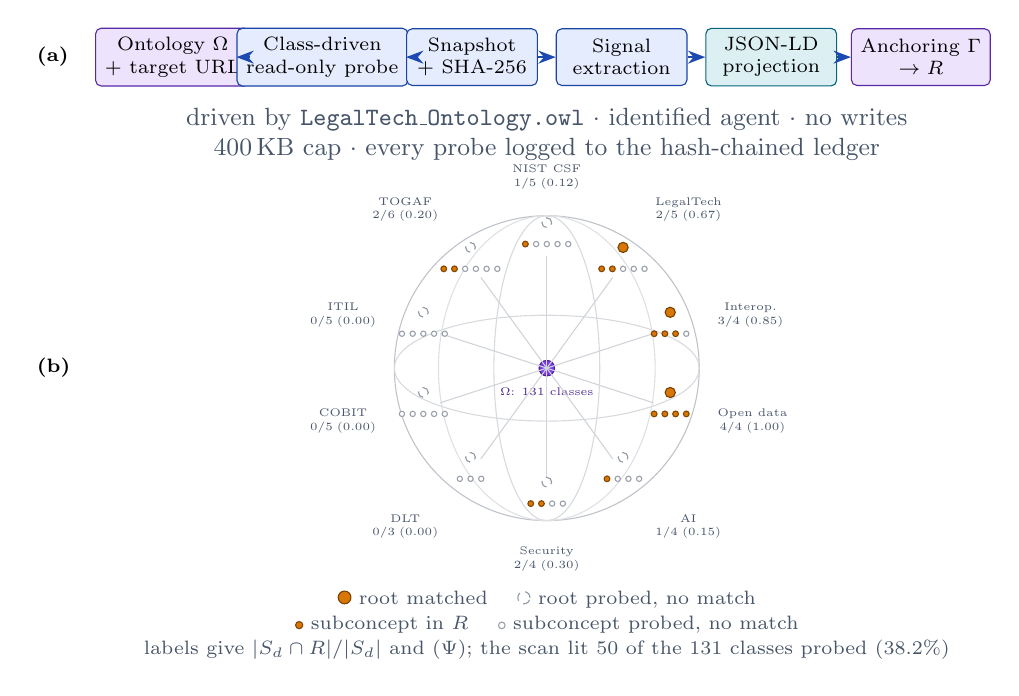
\begin{tikzpicture}[scale=1, transform shape,
  stg/.style={draw=lsBlue!70!black, rounded corners=2pt, minimum width=1.66cm, minimum height=0.72cm, align=center, font=\scriptsize, fill=lsBlue!12},
  arr/.style={-{Stealth[length=2.2mm]}, thick, lsBlue!75!black},
  rlit/.style={circle, fill=lsAmber, draw=lsAmber!55!black, inner sep=0pt, minimum size=4.6pt},
  rdim/.style={circle, fill=white, draw=lsSlate!60, densely dashed, inner sep=0pt, minimum size=4.4pt},
  slit/.style={circle, fill=lsAmber, draw=lsAmber!60!black, inner sep=0pt, minimum size=2.6pt},
  sdim/.style={circle, fill=white, draw=lsSlate!55, inner sep=0pt, minimum size=2.4pt},
  cst/.style={font=\tiny, text=lsSlate, align=center}]
\node[stg, draw=lsViolet!70!black, fill=lsViolet!14] (s0) at (0,0) {Ontology $\Omega$\\\scriptsize + target URL};
\node[stg] (s1) at (1.90,0) {Class-driven\\read-only probe};
\node[stg] (s2) at (3.80,0) {Snapshot\\+ SHA-256};
\node[stg] (s3) at (5.70,0) {Signal\\extraction};
\node[stg, draw=lsCyan!70!black, fill=lsCyan!14] (s4) at (7.60,0) {JSON-LD\\projection};
\node[stg, draw=lsViolet!70!black, fill=lsViolet!14] (s5) at (9.50,0) {Anchoring $\Gamma$\\$\rightarrow R$};
\foreach \a/\b in {s0/s1,s1/s2,s2/s3,s3/s4,s4/s5}{\draw[arr] (\a) -- (\b);}
\node[font=\small, text=lsSlate, anchor=north, align=center] at (4.75,-0.52)
  {driven by \texttt{LegalTech\_Ontology.owl} $\cdot$ identified agent $\cdot$ no writes\\
   400\,KB cap $\cdot$ every probe logged to the hash-chained ledger};
\node[font=\scriptsize\bfseries, anchor=west] at (-1.85,0) {(\textbf{a})};

% ── (b) constelación : conteos |S_d∩R|/|S_d| por la ontología (Tabla 3).
\begin{scope}[shift={(4.75,-3.95)}, scale=0.80]
\draw[lsSlate!35] (0,0) circle (2.42);
\draw[lsSlate!22] (0,0) ellipse (2.42 and 0.84);
\draw[lsSlate!22] (0,0) ellipse (0.84 and 2.42);
\draw[lsSlate!18] (0,0) ellipse (1.72 and 2.42);
\node[circle, fill=lsViolet, draw=lsViolet!60!black, inner sep=0pt, minimum size=7pt] at (0,0) {};
\node[font=\tiny, text=lsViolet!60!black, anchor=north] at (0,-0.18) {$\Omega$: 131 classes};
\foreach \a in {90,54,18,-18,-54,-90,-126,-162,162,126}{\draw[lsSlate!25] (0,0) -- (\a:1.78);}
\lsconst{-18}{rlit}{-1.5/slit,-0.5/slit,0.5/slit,1.5/slit}
\node[cst, anchor=west] at (-18:2.72) {Open data\\4/4\;(1.00)};
\lsconst{18}{rlit}{-1.5/slit,-0.5/slit,0.5/slit,1.5/sdim}
\node[cst, anchor=west] at (18:2.72) {Interop.\\3/4\;(0.85)};
\lsconst{54}{rlit}{-2/slit,-1/slit,0/sdim,1/sdim,2/sdim}
\node[cst, anchor=south west] at (54:2.72) {LegalTech\\2/5\;(0.67)};
\lsconst{90}{rdim}{-2/slit,-1/sdim,0/sdim,1/sdim,2/sdim}
\node[cst, anchor=south] at (90:2.72) {NIST CSF\\1/5\;(0.12)};
\lsconst{126}{rdim}{-2.5/slit,-1.5/slit,-0.5/sdim,0.5/sdim,1.5/sdim,2.5/sdim}
\node[cst, anchor=south east] at (126:2.72) {TOGAF\\2/6\;(0.20)};
\lsconst{162}{rdim}{-2/sdim,-1/sdim,0/sdim,1/sdim,2/sdim}
\node[cst, anchor=east] at (162:2.72) {ITIL\\0/5\;(0.00)};
\lsconst{-162}{rdim}{-2/sdim,-1/sdim,0/sdim,1/sdim,2/sdim}
\node[cst, anchor=east] at (-162:2.72) {COBIT\\0/5\;(0.00)};
\lsconst{-126}{rdim}{-1/sdim,0/sdim,1/sdim}
\node[cst, anchor=north east] at (-126:2.72) {DLT\\0/3\;(0.00)};
\lsconst{-90}{rdim}{-1.5/slit,-0.5/slit,0.5/sdim,1.5/sdim}
\node[cst, anchor=north] at (-90:2.72) {Security\\2/4\;(0.30)};
\lsconst{-54}{rdim}{-1.5/slit,-0.5/sdim,0.5/sdim,1.5/sdim}
\node[cst, anchor=north west] at (-54:2.72) {AI\\1/4\;(0.15)};
\end{scope}
\node[font=\scriptsize\bfseries, anchor=west] at (-1.85,-3.95) {(\textbf{b})};
\node[font=\scriptsize, text=lsSlate, anchor=north, align=center] at (4.75,-6.65)
  {\tikz\node[rlit]{};~root matched \quad \tikz\node[rdim]{};~root probed, no match\\[1pt]
   \tikz\node[slit]{};~subconcept in $R$ \quad \tikz\node[sdim]{};~subconcept probed, no match\\[1pt]
   labels give $|S_d\cap R|/|S_d|$ and $(\Psi)$; the scan lit 50 of the 131 classes probed (38.2\%)};
\end{tikzpicture}

\caption{The GET-SDS acquisition process, driven by the ontology. (\textbf{a}) Pipeline: $\Omega$ declares what is worth looking for, the probe fetches only that, and every step is written to the hash-chained ledger. (\textbf{b}) The same ontology as a celestial sphere: each dimension is a constellation whose large marker is its root $r_d$ and whose small markers are its subconcepts $S_d$. The field starts uniformly dim and the scan lights only what it matches, so the figure shows the shadow being raised rather than its final state alone. Open data closes completely; interoperability and LegalTech match at the root and in part of their detail; TOGAF, NIST~CSF, security and AI match only below the root---an incomplete practice; COBIT, ITIL and DLT stay dark---an absent one. Marker positions are schematic; the counts are exact.\label{fig:getsds}}
\end{figure}

    Algorithm~\ref{alg:sds} states the procedure executed on every run, so that a third party can re-run it at a new cut-off date and compare artefacts.

\begin{figure}[H]
\centering
\begin{minipage}{\textwidth}
\footnotesize
\refstepcounter{algo}\label{alg:sds}%
\rule{\textwidth}{0.6pt}\\[2pt]
\textbf{Algorithm \thealgo:} Digital shadow generation and semantic validation\\[-6pt]
\rule{\textwidth}{0.4pt}
\begin{tabbing}
xxx\=xx\=\kill
\textbf{Input:} seed targets $T$; ontology $\Omega$; dimensions $D$; weights $(w_r,w_s)$\\
\textbf{Output:} shadow $\Delta$; coverage set $R$; per-dimension $\Psi,\mathrm{sds},\delta$; index $L$\\[2pt]
1.\> derive the probe set $P$ from $\Omega$: each class $c\in C$ contributes its observable evidence pattern\\
2.\> \textbf{for each} $\tau\in T$, \textbf{for each} $\rho\in P$: fetch read-only (identified agent, 400\,KB cap);\\
\> store snapshot; log the probing class, URL, UTC timestamp, bytes, latency, SHA-256 and match outcome\\
3.\> verify integrity: re-hash each snapshot, abort on mismatch, append the run to the ledger\\
4.\> extract deterministic signals from the markup (generator, legacy links, JSON-LD, API)\\
5.\> project signals into $\Delta=G(V,E,\lambda)$ and serialise as JSON-LD with the \texttt{@context} of $\Omega$\\
6.\> \textbf{for each} $v\in V$: resolve $\Gamma(v)\subseteq C$ via \texttt{maltg:mapsTo}; reject dangling identifiers\\
7.\> $R \leftarrow \bigcup_{v\in V}\Gamma(v)$\hfill\textit{// Eq.~\eqref{eq:coverage-set}}\\
8.\> \textbf{for each} $d\in D$: $\Psi(d)\leftarrow$ Eq.~\eqref{eq:psi}; then $\mathrm{sds}(d)$ and $\delta(d)$ by Eq.~\eqref{eq:delta}\\
9.\> aggregate to $\Psi_{\mathrm{global}}$ (Eq.~\eqref{eq:global}); $L\leftarrow$ band; sort $D$ by $\delta$ descending\\
10.\> persist the dated artefact with the ontology and shadow digests
\end{tabbing}
\vspace{-6pt}\rule{\textwidth}{0.6pt}
\end{minipage}
\end{figure}

\section{Case Study and Results}
\label{sec:results}
    The study applies LegalShadow to the public digital ecosystem of the Ecuadorian Judiciary Council (\texttt{funcionjudicial\-.gob\-.ec}) and validates the resulting shadow against the full ontology (131 classes, 144 relations, 14 cross-cutting), contrasted with a synthetic \emph{positive control}: a 39-component shadow authored to saturate the engine, whose role is to establish that the metric can approach unity on a well-anchored artefact.
    
%❱❱ EDITOR 3.2(c) — TRANSPARENCIA DE σ: rúbrica versionada de cinco niveles observables
%❱❱   y distinción declared/observed.
    \textbf{Scoring protocol.} 
    The ontological scores $\sigma$ are derived from a versioned rubric that defines five evidence-based maturity levels (0, 25, 50, 75, 100) for each dimension, ensuring transparent and auditable evaluation. Scores lacking supporting evidence are classified as \emph{declared} rather than \emph{observed}, distinguishing institutional self-description from empirically verifiable coverage. Rubrics, evidence sources, and generated shadows are versioned to support traceability and review (Section~\ref{sec:conclusions}).

    The two metrics used in the model have different epistemic roles. While $\mathrm{onto}(d)$ depends on expert assessment and may vary with alternative interpretations of the rubric, $\Psi(d)$ is fully deterministic, being computed directly from the rule set and stored evidence. This separation enables partial replication: reviewers may recompute $\Psi(d)$ from the published artefacts and, if desired, apply alternative $\mathrm{onto}(d)$ values to obtain their own prioritization. Consequently, the framework preserves reproducibility of observed coverage while allowing flexibility in the interpretation of maturity levels.

%❱❱ EDITOR 3.1(a) — Ventana de observación declarada explícitamente (17 corridas,
%❱❱   2 jul–4 ago 2026) y desambiguación de las tres cardinalidades.
    \textbf{Evidence corpus.} 
    Over 17 dated runs between 2 July and 4 August 2026 the acquisition tier issued 187 read-only requests, of which 170 succeeded (90.9\%). Re-hashing every stored snapshot against its manifest yields \textbf{170 matches and 0 mismatches}: full integrity of the evidence base.
    
    Three cardinalities appear here and measure different things: a \emph{run} is one pass of the protocol; a \emph{shadow regeneration} is a run that also rebuilt $\Delta$ end to end, of which there are five; a \emph{ledger entry} records a run, a verification or a methodological decision, hence their larger number. Latencies (median 788.5~ms, p95 954.4~ms, range 67--2810~ms) confirm the probe imposes negligible load, a design requirement of the ethical protocol \cite{Krotov2020}.

    \textbf{Institutional shadow and declarative maturity.} 
    The shadow from the 4 August run contains \textbf{34 components, 32 flows and 7 architectural layers} anchored to 11 seed sources, with anchoring \emph{total and referentially closed}: every component carries at least one anchor (mean 2.00, max 4) and all 50 distinct references resolve, with zero dangling identifiers. Signals show a modern portal on a generic content manager still surfacing 16 legacy links (6 JSF, 10 PHP), a confirmed case-consultation SPA with no documented public API, and the total absence of embedded JSON-LD despite declarative references to open data policies---exactly the gap between nominal publication and effective reuse reported in the open government literature \cite{Janssen2012,Attard2015}. The assessment over the four dimensions for which the institution publishes declarative evidence gives a global index of \textbf{46/100}, which $L$ places at Level 3 (``Defined''): data and semantic interoperability 28, integration architecture 42, declared transformation 55, regulatory compliance 58. Both this index and the coverage figures reported below were invariant across the five regenerated shadows: the only signal that drifted in the series was the legacy PHP count (13~$\rightarrow$~10 between 5 and 30 July), attributable to content editing on the observed portal, and that signal anchors no ontology class, so the coverage set $R$---and with it $\Psi_{\mathrm{global}}$---did not change.

    \textbf{Ten-dimension semantic validation.} Applying the engine of Section~\ref{sec:formal} to the same real shadow (Table~\ref{tab:validation}, Figure~\ref{fig:gaps}) gives $\Psi_{\mathrm{global}}=25.8/73.9=\mathbf{0.349}$: the shadow materialises only 34.9\% of the maturity the ontology prescribes, leaving an aggregate gap of 48.2 points (65.1\%). The positive control reaches $\Psi_{\mathrm{global}}=66.9/73.9=90.4\%$ with a residual gap of 7.1. This rules out a ceiling artefact in the scoring engine and shows that the low real coverage is a property of the observed ecosystem rather than of the instrument; it does not, on its own, establish construct validity, since the control was authored by the same team (Section~\ref{sec:conclusions}).

    A result visible only through the shared apparatus is that both shadows light almost the same number of stars---50 of 131 for the real shadow against 51 for the control---yet their global coverage differs by a factor of 2.6. Coverage \emph{breadth} is not what $\Psi$ measures: \emph{which} concepts are anchored matters far more than how many. The control spreads its 51 anchors across all ten dimensions; the real ecosystem concentrates its 50 in open data, interoperability and LegalTech, leaving whole dimensions untouched. A naive count of evidenced nodes would have rated the two artefacts equivalent.

%❱❱ EDITOR 4(a) — Descripción en el texto corrido de la figura de brechas.
    Figure~\ref{fig:gaps} renders the same table as three series ordered by decreasing $\delta$---light bars for what the ontology prescribes, dark for what the shadow delivers, dashed line for the difference---so that reading left to right gives the agenda directly. The shape carries the argument: the bar series converge only at the right-hand end, where open data and interoperability sit, and diverge almost completely on the left, where the enterprise frameworks are.

    Three dimensions have \emph{zero} coverage because neither root nor subconcepts appear in $R$: service management (ITIL, $\delta=79.5$), control (COBIT, $\delta=62.7$) and distributed ledger ($\delta=52.4$). Four more are lit only below the root---AI, NIST CSF, security posture and TOGAF---which is a different condition and calls for different remediation. The single largest gap is AI integration ($\delta=82.4$), where a high ontological score (96.9) is almost entirely unrealised. Conversely open data attains full coverage and interoperability 0.85, reflecting genuine participation in the national open data catalogue.

%❱❱ EDITOR 3.4(c) — CONTRASTE 4 vs 10 DIMENSIONES elevado a párrafo propio y titulado,
%❱❱   tal como pide el editor que se destaque.
    \textbf{The two headline figures do not measure the same thing---and that is the finding.} It is tempting to read 46/100 against 34.9\% as a single quantity assessed twice, and that reading would be wrong. The 46/100 aggregates the \emph{four} dimensions on which the institution itself publishes declarative evidence: data and semantic interoperability, integration architecture, declared transformation, regulatory compliance. $\Psi_{\mathrm{global}}$ spans the \emph{ten} dimensions the ontology prescribes. Neither the scales nor the dimension sets coincide, so the comparison is not a difference of degree but a difference of frame: what an institution reports \emph{on its own terms} versus what its digital surface exposes \emph{on the frameworks' terms}. Read that way the result is sharper rather than weaker. An institution can only report progress on the dimensions it has chosen to instrument; the six dimensions missing from its own assessment---ITIL, COBIT, distributed ledger, AI, NIST CSF and security posture---are, without exception, the ones in which the ontology finds little or no machine-processable trace. The self-assessment is not merely optimistic in value; it is silent exactly where the deficit is.

\begin{table}[H]
\small
\caption{Hierarchical coverage validation of the real institutional shadow, $(w_r,w_s)=(0.40,\,0.60)$. The last column reports the synthetic positive control for the same dimension. Aggregates follow Equation~\eqref{eq:global} with equal $\omega_d$ and are computed on unrounded values; $\Psi_{\mathrm{global}}$ is thus an $\mathrm{onto}$-weighted mean of the $\Psi(d)$ column, whose unweighted mean is 0.329 (real) and 0.900 (control).\label{tab:validation}}
\begin{tabularx}{\textwidth}{Xcccccc}
\toprule
\textbf{Dimension} & $\mathbf{onto(d)}$ & \textbf{Root} & $\mathbf{\Psi(d)}$ & $\mathbf{sds(d)}$ & $\boldsymbol{\delta}\mathbf{(d)}$ & $\mathbf{\Psi}$ \textbf{ctrl}\\
\midrule
AI integration            & 96.9 & No  & 0.150 & 14.5 & \textbf{82.4} & 0.85\\
Service management (ITIL) & 79.5 & No  & 0.000 & 0.0  & \textbf{79.5} & 1.00\\
Resilience (NIST CSF)     & 72.0 & No  & 0.120 & 8.6  & 63.4 & 1.00\\
Control (COBIT)           & 62.7 & No  & 0.000 & 0.0  & 62.7 & 1.00\\
Security posture          & 80.4 & No  & 0.300 & 24.1 & 56.3 & 1.00\\
Distributed ledger        & 52.4 & No  & 0.000 & 0.0  & 52.4 & 0.85\\
Governance (TOGAF)        & 60.3 & No  & 0.200 & 12.1 & 48.2 & 0.70\\
LegalTech domain          & 75.5 & Yes & 0.673 & 50.8 & 24.7 & 0.60\\
Interoperability          & 81.2 & Yes & 0.850 & 69.0 & 12.2 & 1.00\\
Open data                 & 78.5 & Yes & 1.000 & 78.5 & 0.0  & 1.00\\
\midrule
\textbf{Global (Eq.~\eqref{eq:global}, $\mathrm{onto}$-weighted)} & \textbf{73.9} & 3/10 & \textbf{0.349} & \textbf{25.8} & \textbf{48.2} & \textbf{0.904}\\
\bottomrule
\end{tabularx}
\end{table}

\begin{figure}[H]
\centering
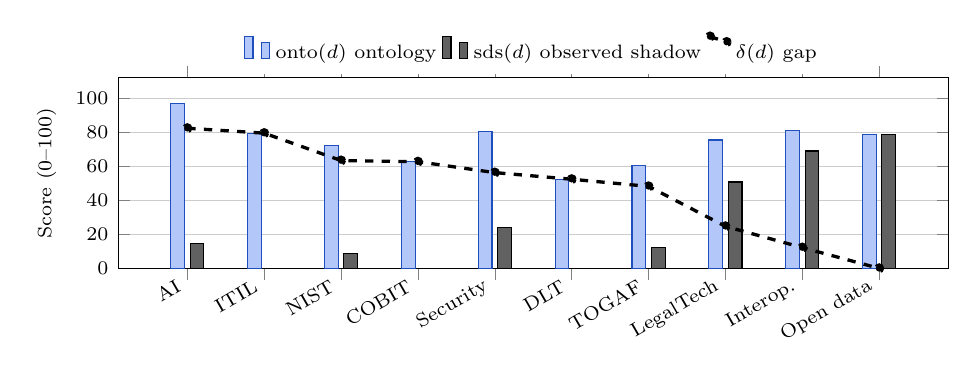
\begin{tikzpicture}
\begin{axis}[
  ybar,
  width=\textwidth, height=4.0cm,
  bar width=5pt,
  ymin=0, ymax=112,
  ylabel={Score (0--100)},
  ylabel style={font=\scriptsize},
  symbolic x coords={AI,ITIL,NIST,COBIT,Security,DLT,TOGAF,LegalTech,Interop.,Open data},
  xtick=data,
  x tick label style={rotate=30, anchor=east, font=\scriptsize},
  ytick={0,20,40,60,80,100},
  yticklabel style={font=\scriptsize},
  legend style={font=\scriptsize, at={(0.5,1.02)}, anchor=south, legend columns=3, draw=none},
  ymajorgrids, major grid style={black!20},
]
\addplot+[draw=lsBlue!80!black, fill=lsBlue!35] coordinates
  {(AI,96.9) (ITIL,79.5) (NIST,72.0) (COBIT,62.7) (Security,80.4) (DLT,52.4) (TOGAF,60.3) (LegalTech,75.5) (Interop.,81.2) (Open data,78.5)};
\addplot+[draw=black, fill=black!62] coordinates
  {(AI,14.5) (ITIL,0) (NIST,8.6) (COBIT,0) (Security,24.1) (DLT,0) (TOGAF,12.1) (LegalTech,50.8) (Interop.,69.0) (Open data,78.5)};
\addplot[sharp plot, very thick, dashed, black, mark=*, mark size=1.2pt] coordinates
  {(AI,82.4) (ITIL,79.5) (NIST,63.4) (COBIT,62.7) (Security,56.3) (DLT,52.4) (TOGAF,48.2) (LegalTech,24.7) (Interop.,12.2) (Open data,0)};
\legend{$\mathrm{onto}(d)$ ontology, $\mathrm{sds}(d)$ observed shadow, $\delta(d)$ gap}
\end{axis}
\end{tikzpicture}
\caption{Ontological versus effective maturity of the real institutional shadow, ordered by decreasing gap. The dashed line traces $\delta(d)$ and constitutes the remediation agenda.\label{fig:gaps}}
\end{figure}

%% ============================================================
\section{Discussion and Conclusions}
\label{sec:conclusions}

%❱❱ ESTRUCTURA: cinco párrafos. Se fusionaron "Measurement implications" e
%❱❱   "Improvement opportunities" dentro del hallazgo reflexivo (decían lo mismo),
%❱❱   la transferibilidad de "Limitations" se absorbió en "External validity", y
%❱❱   "Contribution" se integró en las conclusiones. Sin pérdida de contenido.

\textbf{Declarative maturity vs. semantic coverage.}
    Although the institution attains a maturity score of 46/100, its observable ecosystem materialises only 34.9\% of the governance dimensions defined by the referenced frameworks. The results reveal a gap between declared governance and machine-processable evidence, highlighting dimensions that remain only partially represented or entirely absent on the public digital surface.

%❱❱ EDITOR 3.5 — HALLAZGO REFLEXIVO desarrollado en sus dos vertientes:
%❱❱   (i) limitación metodológica: la cobertura es propiedad conjunta del ecosistema y
%❱❱       de sus prácticas de publicación, de modo que un Ψ bajo no distingue gobernanza
%❱❱       débil de divulgación insuficiente;
%❱❱   (ii) recomendación concreta para instituciones públicas: JSON-LD embebido,
%❱❱       documentar APIs y publicar un manifiesto de gobernanza legible por máquina.
\textbf{Reflexive finding and implications.}
    The main gap identified is the absence of embedded JSON-LD and documented public APIs: the institution lacks the very instrument---structured data---that the shadow needs in order to represent it. This carries a methodological consequence. Coverage is a joint property of the ecosystem and of its publication practices, so any external instrument of this family resolves governance only to the granularity at which the institution has chosen to structure its public surface. A low $\Psi$ therefore cannot distinguish weak governance from governance that is real but undisclosed in machine-readable form, and semantic publication becomes a determinant of measurable coverage in its own right \cite{Guha2016}. Two corollaries follow: no refinement of $\Gamma$ removes this bound---only the institution can, by publishing---and longitudinal use must control for the fact that adopting semantic markup would raise measured coverage with no change in underlying governance.

    The prescriptive consequence is that the highest-leverage remediation is also the cheapest. Embedding \texttt{schema.org} JSON-LD, documenting the public services that demonstrably already exist behind the single-page application, and publishing a machine-readable governance statement declaring frameworks in use, owners and review cycles would together improve discoverability, interoperability, transparency and external reuse of judicial data \cite{Guha2016,Attard2015,Wilkinson2016}. None of these requires modifying internal governance processes; all three expand what can be audited from the public surface, and would complement---rather than replace---an internal assessment conducted with privileged access to the same ecosystem.

%❱❱ EDITOR 3.1(b) — VALIDEZ EXTERNA: se acota qué generaliza y qué no, y se da el
%❱❱   protocolo de transferencia en cuatro pasos a otros ecosistemas judiciales.
\textbf{External validity and transferability.}
    The empirical results are specific to a single institution and a one-month observation window of 17 dated runs; values such as 46/100 and $\Psi_{\mathrm{global}}=34.9\%$ describe the Ecuadorian Judiciary Council and should be interpreted only within that context. While the observed gap between declared maturity and semantic coverage aligns with findings on publication and reuse limitations in open-data ecosystems \cite{Janssen2012,Attard2015,Neumaier2016}, its generality is a hypothesis that only multi-institutional study can test. The transferable element is the instrument itself: the ontology $\Omega$ and its governance frameworks remain largely reusable, and adaptation concentrates on localising the anchoring rules of $\Gamma$ to national infrastructures.

    Transfer takes four steps, of which only the second costs anything. (1)~Replace the seed file: the target is already a parameter. (2)~Localise the rule table of $\Gamma$: roughly a fifth of the rules key on national artefacts---the Ecuadorian catalogue, national interoperability schemes---and must be re-expressed against equivalent infrastructure, the one step demanding domain knowledge and the real obstacle to naive reuse. (3)~Leave $\Omega$ and its rubric unchanged where the frameworks are international, which covers eight of ten dimensions. (4)~Compare only $\Psi$ and $\delta$ across institutions, never raw signal counts, since portal technologies differ. Comparability rests on holding the ontology fixed while the rule table varies---the discipline that makes urban twins comparable across cities \cite{Shahat2021,Haraguchi2024}---and whether it survives contact with a second jurisdiction is untested.

%❱❱ EDITOR 3.1(c)+3.2(d) — Limitaciones: cota inferior observable, juicio experto en σ
%❱❱   pendiente de validación independiente y alcance del control positivo.
\textbf{Limitations.}
    Results represent \emph{observable} maturity and therefore constitute a lower bound on actual institutional capabilities: dimensions such as ITIL or COBIT may operate internally without public trace, so their zero coverage measures published evidence rather than practice. Dimension weights and ontological scores incorporate expert judgement and await independent validation---no Delphi round, content-validity ratio \cite{Lawshe1975} or inter-rater agreement has yet been computed---so the absolute value of $\delta$ carries unquantified judgement even though $\Psi$ does not. The synthetic control is a positive control only: authored by the same team to saturate the engine, it bounds instrument artefacts but does not establish construct validity. Signal detection also depends on portal markup stability, which the cryptographic record attenuates without eliminating.

\textbf{Conclusions and future work.}
    LegalShadow applies the digital shadow paradigm to judicial technological ecosystems by combining public web evidence, semantic representation through a governance ontology, and quantitative analysis based on $\Psi$ and $\delta$. The metric operationalises ontology--artefact alignment with a bounded and interpretable measure of semantic coverage \cite{Karabulut2024}, and its root/subconcept structure separates absent, partial and mature implementation states---diagnostic insight that an aggregate maturity score cannot express. Every figure reported here is recomputable by a third party from the published rubric, rule table and dated artefacts, which is what turns the instrument into an audit rather than an assessment. The approach is built on enterprise standards, HTTP-based acquisition and global JSON-LD vocabularies, so adaptation to other contexts mainly requires revising the anchoring rules of $\Gamma$. Future work includes multi-institutional studies with full $\Psi/\delta$ evaluation, independent elicitation of dimension weights, ontology alignment to expand semantic coverage \cite{Hogan2021}, assisted decision support under MAPE-K principles \cite{Kephart2003}, and behavioural indicators to complement structural assessment \cite{Medvedeva2020}. Comparisons across institutions and over time could further extend its analytical value \cite{Shahat2021,Haraguchi2024}.


\authorcontributions{
    Conceptualisation, methodology, software, 
    investigation, data curation and
    writing---original draft preparation,               P.M.P.-A.;
    validation and formal analysis,                     P.M.P.-A. and E.J.S.-C.;
    writing---review and editing, and visualisation,    P.M.P.-A., E.J.S.-C. and V.V.V.-B.;
    supervision and project administration,             E.J.S.-C.
    All authors have read and agreed to the published version of the manuscript.
}
\funding{This research received no external funding.}
\dataavailability{
    All artefacts of this study---the LegalShadow source code, the OWL governance ontology, the versioned scoring rubric that fixes $\mathrm{onto}(d)$, the \emph{signal}$\rightarrow$\emph{class} rule table that constitutes $\Gamma$, the dated JSON-LD shadows and the SHA-256 evidence manifests---are openly available without restriction at Zenodo \cite{paccha2026zenodo} and at \texttt{https://github.com/patmic/ArchLab}. 
    
    Publishing the rubric and the rule table alongside the snapshots is what makes the two-level replication described in Section~\ref{sec:results} possible: $\Psi$ can be recomputed without rerunning acquisition, and $\mathrm{onto}$ can be replaced by a reviewer's own values. 
    %The evidence base reported here corresponds to ledger head \texttt{6c7d2847932a606f}, which any third party can recompute from the published manifests. Observed data originate exclusively from public resources of the Ecuadorian Judiciary Council.
    The code and instructions to reproduce the setup are available at:
    \begin{itemize}
        \item git clone https://github.com/patmic/ArchLab
        \item docker compose up -d -{}-build
        \item access the dashboard at http://localhost:8080
    \end{itemize}
}
\institutionalreview{Not applicable.}
\informedconsent{Not applicable.}
\acknowledgments{The authors acknowledge the open-source ontology engineering ecosystem
(\texttt{rdflib}, \texttt{pyvis}, OWLready2).}
\conflictsofinterest{The authors declare no conflicts of interest.}

\begin{adjustwidth}{-\extralength}{0cm}
\reftitle{References}
\bibliography{ICI2ST_LegalShadow_Ref}
\end{adjustwidth}

\PublishersNote{}
\end{document}
